\chapter{Results}
\section{Overview}
This chapter presents the validation process and results of the processes outlined in the 
Methodology (Chapter 
\ref{sec:methodology}). The results are organised by operation. Each section
discusses the correctness and computational performance of an algorithm. Additionally implementation 
decisions for each of the stages are compared for both their speed and accuracy. The results are 
presented as plots, and are accompanied by a discussion of their implications for the design 
of the radar processing pipeline in the following chapter. 

Before the per stage performance is presented, a holistic view of the pipeline's performance is
given, including the ablation study on each of the hardware devices and field trial results.  

The pipeline demonstrates full real-time multi-target tracking functionality on each of the three
hardware platforms: the desktop workstation, the NVIDIA Xavier 
AGX, and the NVIDIA Xavier NX. Best case, the desktop workstation 
can run the whole pipeline at 100 frames per second when the maximum integration size is used, 
the Xavier AGX and NX performed at 500 and 400 frames per second in the same case.  

On top of this, the harness used for visualisation can also run online, 
allowing the user to see the correct 
behaviour of each of the stages of the pipeline in real time. Examples of these visualisations are
for each of these stages are depicted in Appendix Figures  \ref{fig:fft-visual}, 
\ref{fig:cfar-visual}, \ref{fig:cluster-visual}, \ref{fig:angle-visual}, \ref{fig:track-visual1}, 
and \ref{fig:track-visual2}. These figures have been included as a reference for how to visualise
and validate the intermediate stages of a radar processing pipeline. Understanding these 
visualisations is also important for interpreting 
the following figures in this section: \ref{fig:integration-waterfall}, 
\ref{fig:integration-waterfall-orac}, \ref{fig:integration-setup}, \ref{fig:cfar-0.001-waterfall},
\ref{fig:clustering-results}, \ref{fig:angle-2d-plot}, \ref{fig:angle-3d-plot-noise},
\ref{fig:tracking-scenarios}, \ref{fig:tracking-3d-results}.

% Filenames: visual-fft-png, visual-angle.png, visual-cfar.png, visual-cluster.png, visual-track.png
\subsection{Pipeline Ablation Study}

Throughout this chapter, the \emph{integration size} $N$ is the number of
consecutive input chirps that are coherently summed to produce a single output
chirp (record). Equivalently, it is the factor by which the chirp count is
reduced by the integration stage: an integration size of $N$ maps $N$ input
chirps to $1$ output chirp, so the two descriptions --- the number of
summations and the factor of reduction --- refer to the same quantity. Thus an
integration size of $1$ applies no reduction ($256$ output chirps for $256$
input chirps), while the maximum integration size of $256$ applies the greatest
reduction ($1$ output chirp for $256$ input chirps). Larger integration sizes
therefore produce less output data per frame and are the least demanding case
for downstream throughput.

An ablation study is performed on each of the devices 
to determine the contribution of
each stage to the overall latency of the pipeline and their
marginal effects on its throughput. Latency is measured as 
the time between the arrival of a chirp to the capture stage of
the processing subsystem, and the
generation of the output of the pipeline, whatever it may be. 
Throughput is measured as the number of frames processed per 
second after processing 1000 frames each of 52.5 MB in size. 
Dataset DS2 simulates the 
receiver signals of targets across a wide variety of ranges in
high noise. On each trial, the complete pipeline is run up until 
a given terminating stage, for example, label "CFAR" refers to the 
pipeline including all stages up to and including CFAR. 

On the desktop, performance requirements were easily met, and 
a frame rate of above 100 frames per seconds was achieved for the maximum integration 
size of 256, that is 1 output chirp (record) for every 256 input chirps 
(see Figure \ref{fig:ablation-throughput-desktop}). 
One optimisation that was significant was the use of several CPU threads to handle the incoming
frames. Utilising two or four processing buffers allowed the pipeline to maintain 15+ framerate 
even when the integration stage didn't compress the data at all (an integration size of 1, i.e. 
256 output chirps per 256 input chirps). 
Another finding 
made on the desktop was that after CFAR, additional stages only marginally reduced throughput, 
suggesting that host-device transfer, and CPU read/write operations dominated the pipeline's 
compute time. 

On the two Jetson Devices, the device-host memory architecture disallows the asynchronous 
graph execution that was possible on the desktop, limiting CPU operations to one thread. 
The Jetson devices performed with higher performance than the desktop workstation, achieving 
framerates of 25-500 and 20-400 frames per second on the AGX and NX respectively depending on 
integration size (see Figure 
\ref{fig:latency-jetsons}) the latency chart for the desktop workstation and the throughput 
diagrams of the Jetson devices (which will just show the reciprocals of the latencies) is in the 
Appendix \ref{fig:latency-desktop} \ref{fig:throughput-nx} \ref{fig:throughput-agx}.

\begin{figure}
    \centering
    \incfig[0.8]{ablation_throughput_desktop}
    \caption{Pipeline framerate, for 
    different integration sizes (the number of input chirps summed per output 
    chirp, equivalently the factor of reduction). 
    Obtained by finding average frames 
    per second after processing 1000 frames of 52.5 MB each. Each line shows 
    the framerates of the pipeline running up to a given stage. The largest reductions 
    in framerate occur at the integration stage, aggregation stage, and CFAR stage. Frame 
    rate varies from 16 to 100 for the entire pipeline depending on the integration size.}
    \label{fig:ablation-throughput-desktop}
\end{figure}

\begin{figure}
    \centering
    \incfig[0.9]{Ablation_Latency_Breakdown_Jetsons}
    \caption{Pipeline latency breakdown as stages are added for 
    different integration sizes (the number of input chirps summed per output 
    chirp, equivalently the factor of reduction). 
    Split into the processing subsystem
    the detection and tracking subsystem, 
    and a combined view. The capture, integration, aggregation, CFAR and tracking stages 
    are the most significant }
    \label{fig:latency-jetsons}
\end{figure}

\subsection{Tracking Performance at Field Trials}
The radar hardware was taken to an open air field test site in New South Wales 
where it and a target drone were flown in a variety of scenarios. Figure 
\ref{fig:real-world-tracking} depicts one such air to air scenario. 
\begin{figure}
    \centering
    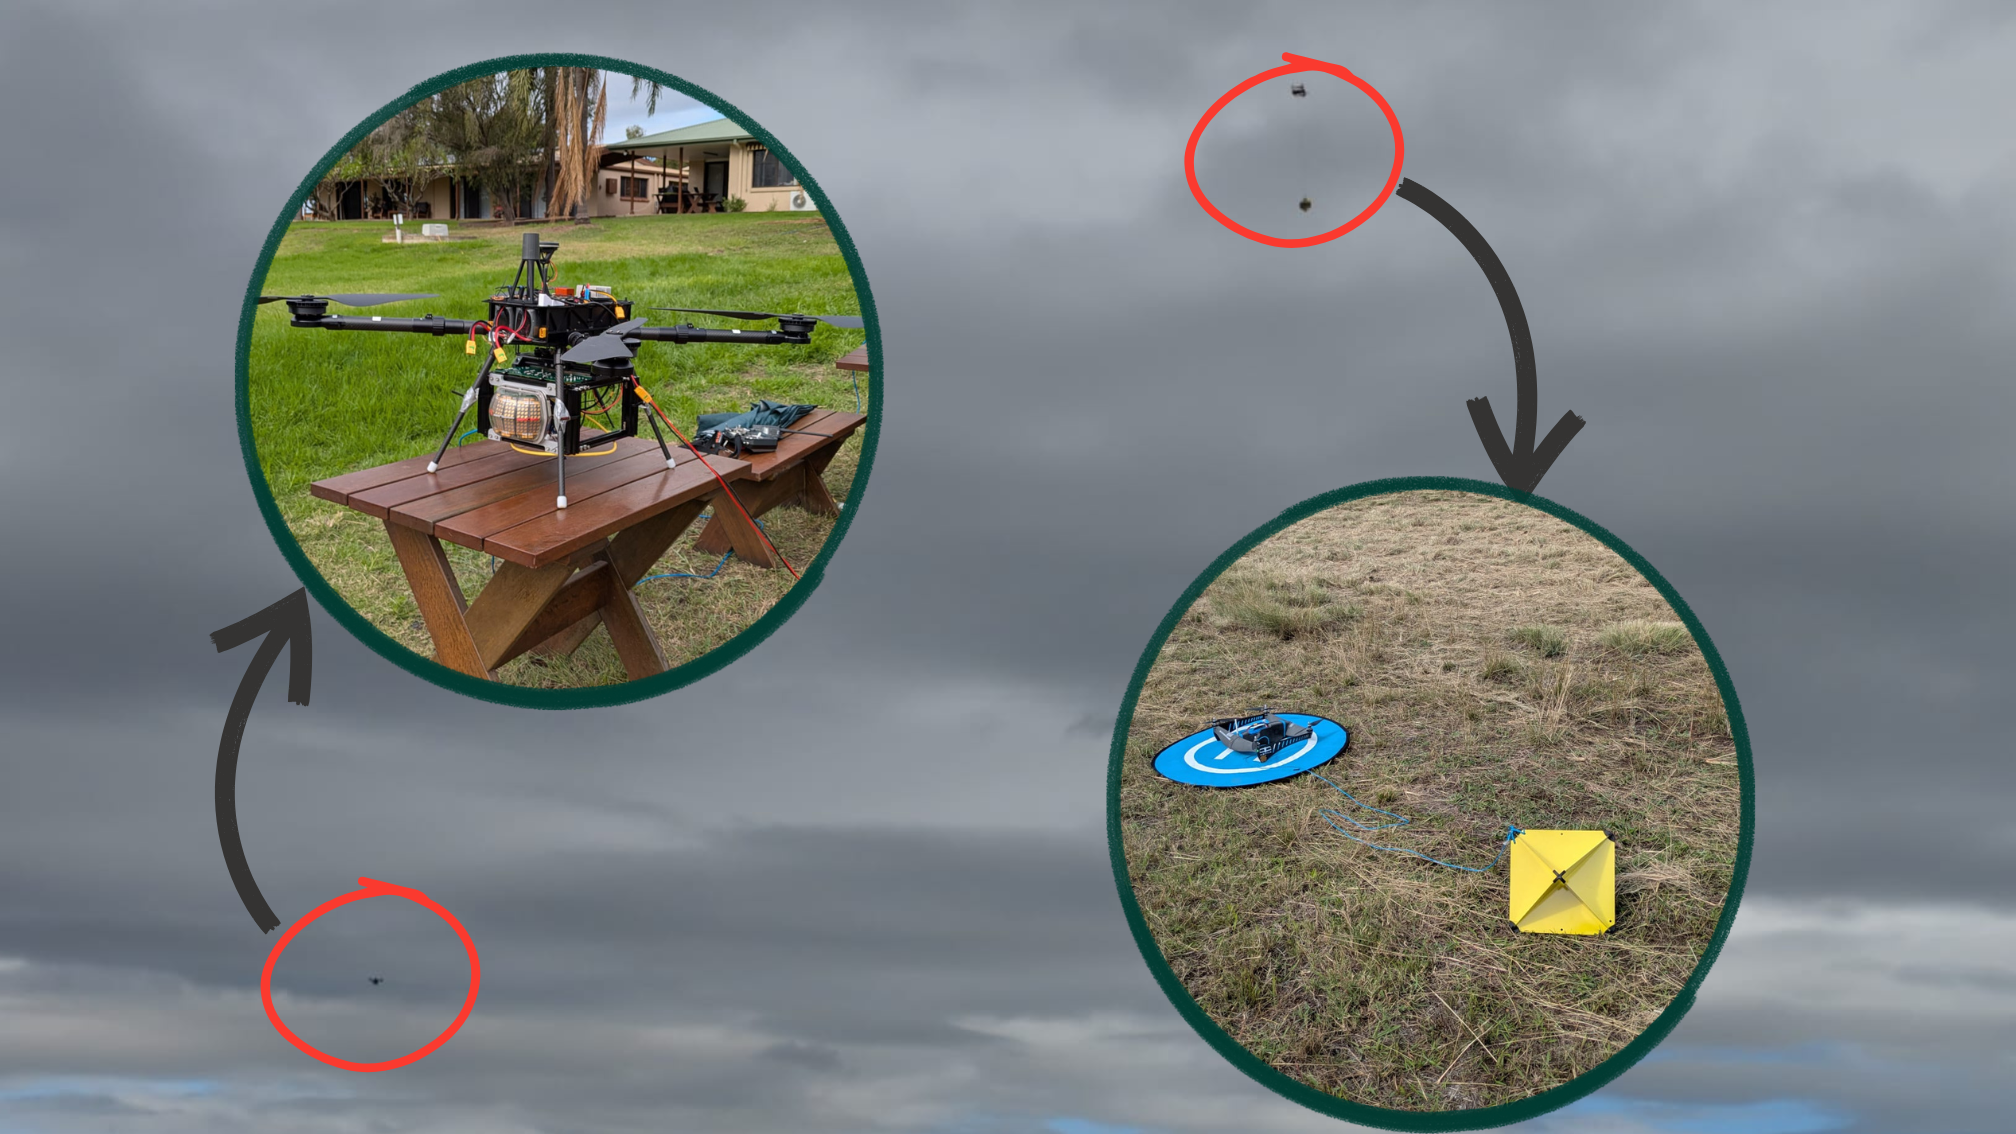
\includegraphics[width=0.6\textwidth]{air-to-air.png}
    \caption{The radar is flown into the air and is pointed at a target drone carrying
    a reflective marker 200m away.}
    \label{fig:real-world-tracking}
\end{figure}

The results of the tracking subsystem failed to produce any tracks of the aerial target, 
due to high coupling between the transmitter and the receiver that saturated the beginning 
of every signal, masking the near-field
where the target was. The radar did detect high cross-section targets 
in the distance (see Figure \ref{fig:field-and-silo}). The detections of these targets are
illustrated in the visualisation of the angle sensing stage
in Figure \ref{fig:points-over-map-singleton}, where detections from the radar line up with
a silo and trees.    

\begin{figure}
    \centering
    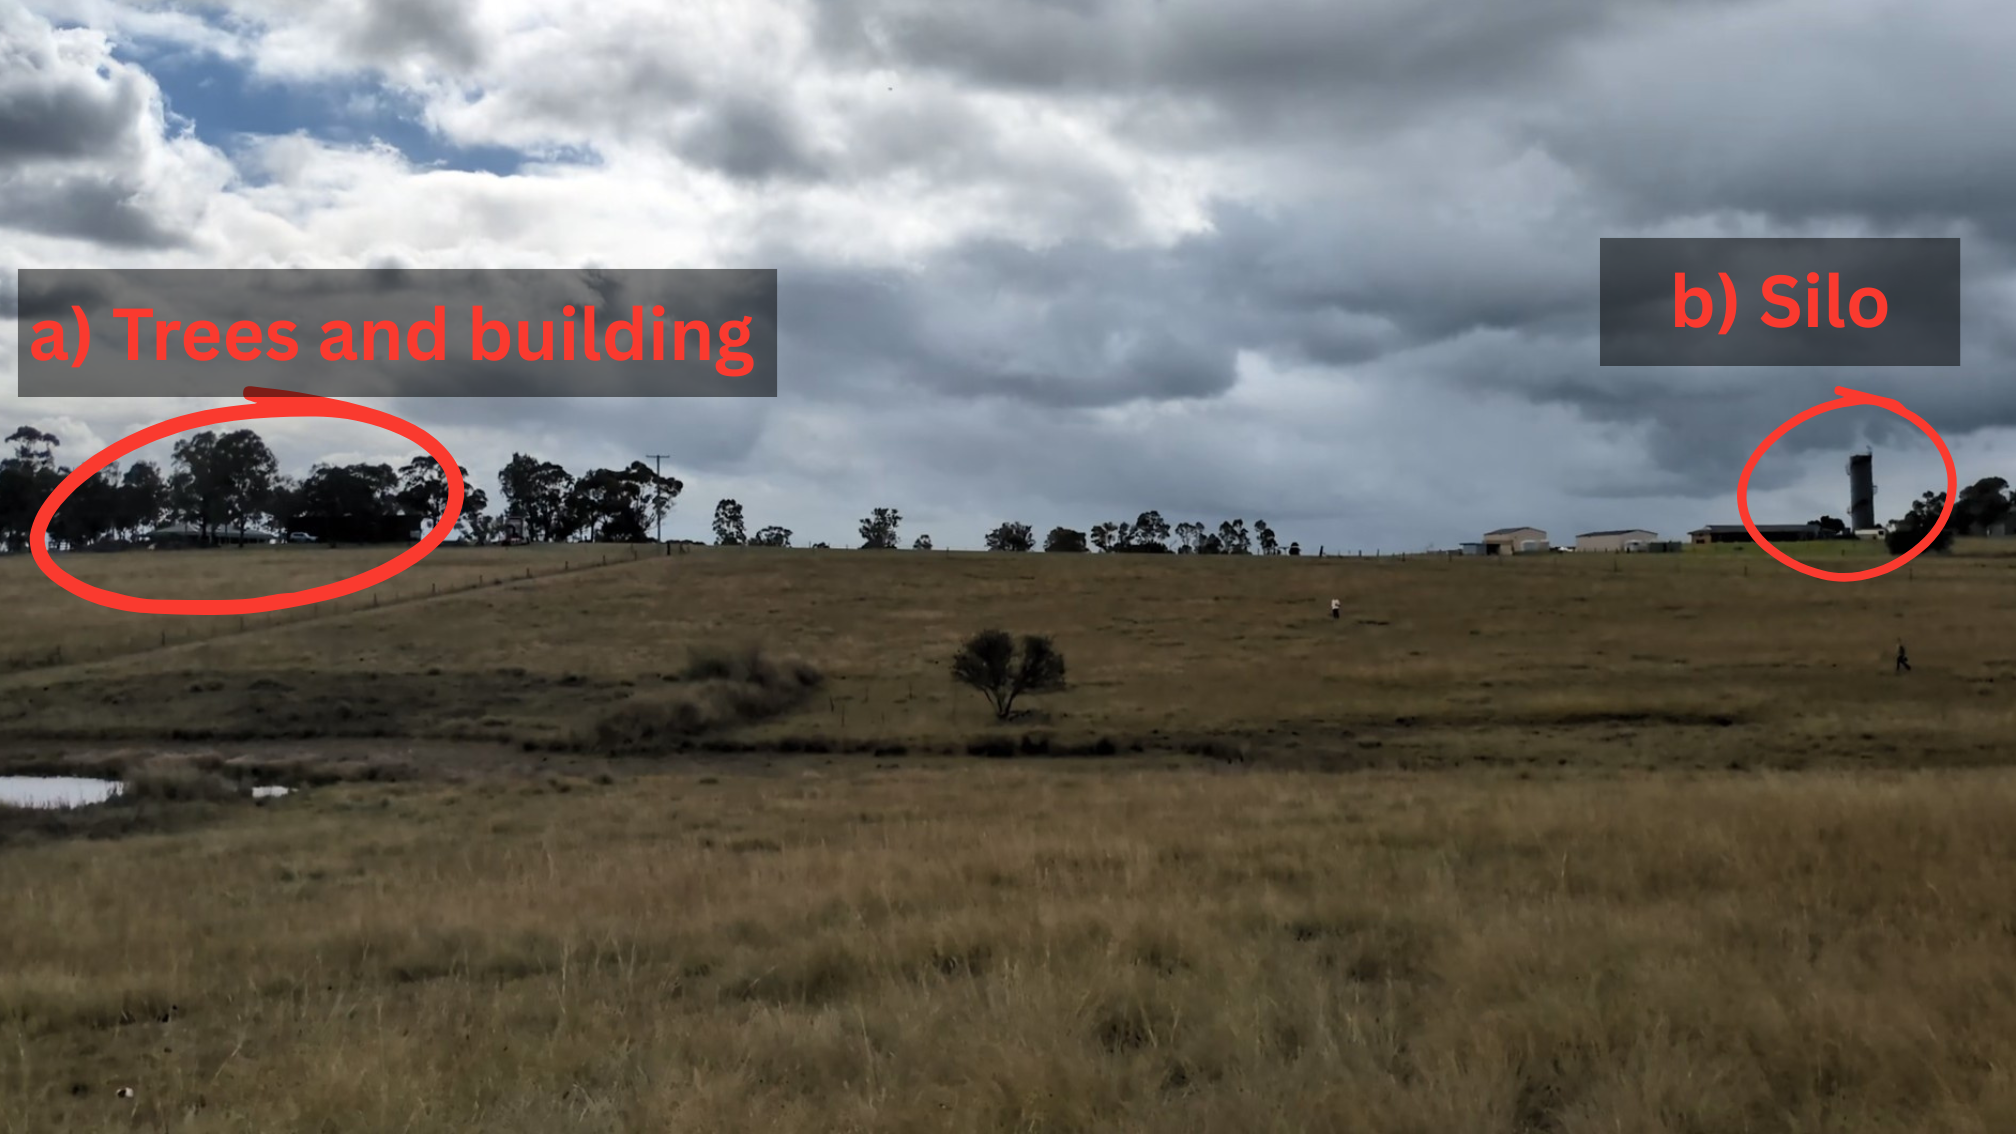
\includegraphics[width=0.6\textwidth]{field-and-silo.png}
    \caption[Radar field of view with silo]{A silo in the distance and a property surrounded by trees are large 
    visible targets for the radar when it is airborne.}
    \label{fig:field-and-silo}
\end{figure}

\begin{figure}
    \centering
    \incfig[0.6]{points-over-map-singleton}
    \caption[Field Trial Silo Detection]{The detected points from the radar are plotted 
    over a map of the area. There is a high correspondence between detected points and
    the three main high cross-section targets in the area: a silo 603 meters away, 
    building 706 m away, and trees surrounding a building 410 meters away. }
    \label{fig:points-over-map-singleton}
\end{figure}

The field trials also provided an opportunity to record realistic noise data, from the open field, and from the radar's own electronics. 
Among the noise was a large DC offset, which produced a peak in the FFT output at 0 Hz, resulting high-power static detections at 
the minimum and maximum range of the radar. This noise was summed with simulated target data to produce D4, one which the whole pipeline was validated 
against in the following section. 

\subsection{Validation in realistic noise}
The pipeline was validated against a dataset D4, which was produced by summing the noise recorded in the field trials with simulated target that
flies in a snaking pattern, sweeping azimuth, elevation and range. Figure \ref{fig:snake} illustrates the ground truth and generated track 
estimations of the snaking target both with and without the realistic noise. Although the signal to noise in both scenarios is held at 0 dB, 
the more irregular noise in the realistic case produces more erratic track estimates, and initiates more false tracks. Despite this,
the tracking subsystem is able to maintain a track of the target.  

\begin{figure}
    \centering
    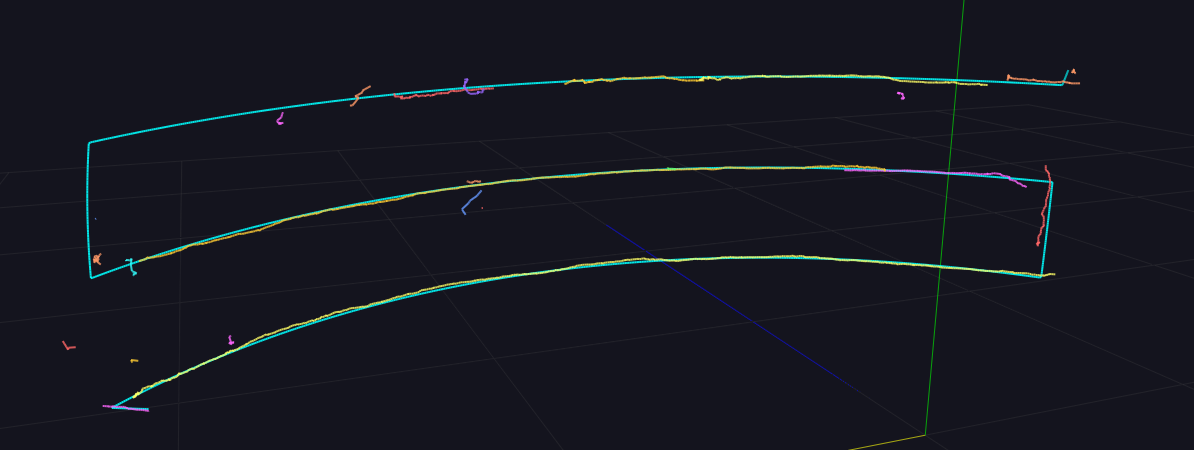
\includegraphics[width=0.7\linewidth]{simulated_snake.png}

    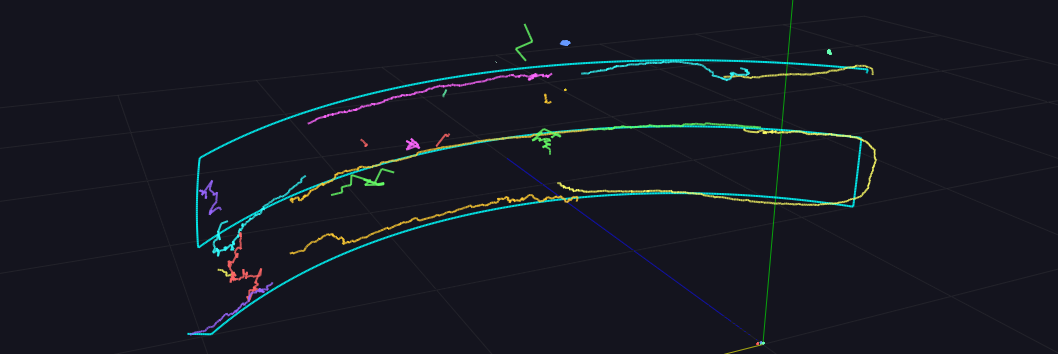
\includegraphics[width=0.8\linewidth]{pseudo_real_snake.png}
    \caption[Tracking a snaking target with and without realistic noise.]{Ground truth
    and track estimates for a target flying a snaking pattern at 0\,dB SNR. The images
    depict just a single range for clarity. The ground truth is depicted in blue while
    a line of a given colour represents an unbroken track. Top: with
    purely simulated noise. Bottom: with realistic noise recorded during field trials
    summed with the simulated target. The realistic noise produces more erratic track
    estimates and initiates more false tracks, though the tracker maintains a track of
    the target throughout.}
    \label{fig:snake}
\end{figure}


\FloatBarrier
\section{Windowing}
The Hann (with $\alpha = 0.5$) and Hamming windows are first evaluated for the prominence of their main lobe and sidelobes
in the frequency domain on the synthetic datasets. Figure \ref{fig:clean filters} illustrates the 
performance of each of the filters on a clear sine wave with no noise. Figure \ref{fig:noisy filters}
illustrates the performance of each of the filters on the noisy simulated data with an SNR of 1.  

\begin{figure}
    \incfig[0.7]{filter_clear_comparison}
    \caption[Window filter comparison on a noise-free signal.]{Results of an \gls{fft} performed on a single frequency signal without noise without a filter,
    with a Hann window, and a Hamming window. Each of the tests correctly produces a peak near
    bin 334, the target range. The no filter option's peak is wider than the filtered options.
    The Hann window performs the best globally, with a 100 dB reduction in power when more than 40
    bin away from the target bin. The Hamming window performs significantly worse globally, with
    only a 70 dB reduction when more than 40 bins away, but has a steeper drop-off near the
    target bin, which may result in better resolution of closely spaced targets.}
    \label{fig:clean filters}
\end{figure}

\begin{figure}
    \incfig[0.7]{filter_noisy_comparison}
    \caption[Window filter comparison at SNR of 1.]{Results of an \gls{fft} performed on a single frequency signal with an SNR of 1 with no
    window filter, with a Hann window filter, and a Hamming window filter. The no filter option's
    spectral leakage acts to deform the peak at bin 334. The Hann and Hamming windows perform similarly
    globally but the Hamming window features a slightly higher peak, and less spectral leakage into
    the adjacent bins.}
    \label{fig:noisy filters}
\end{figure}

In terms of computational performance, the latency contribution of the filters does not significantly 
differ across implementations. Figure \ref{fig:latency} shows the time taken to process
a single frame of 10 000 chirps each with 767 samples, averaged over 50 runs. 

\begin{figure}
    \incfig[0.7]{filter_latency_comparison}
    \caption[Windowing stage latency across implementations.]{Latency contribution of the windowing stage to the overall pipeline. The latency does not
    significantly differ across implementations, with all implementations taking around 9-12 ms to
    process 7 670 000 samples. The insignificant difference in latency between no filter
    and filters suggests that the delay is primarily due to the overhead of handling the data.}
    \label{fig:latency}
\end{figure}

The experiments were then extended to the Blackman, Kaiser, and Taylor windows. Using dataset DS2,
the multi-receiver signal of a target sweep azimuth, elevation and range, fifteen filter 
configurations were applied to the data: \verb|Hann|, \verb|Hamming|, \verb|Blackman|, 
\verb|Kaiser6|, \verb|Kaiser8|, \verb|Kaiser10|, \verb|Kaiser12|, \verb|Taylor1_30|, 
\verb|Taylor2_30|, \verb|Taylor_3_30|, \verb|Taylor_4_30|, \verb|Taylor1_50|, \verb|Taylor2_50|
\verb|Taylor_3_50|, \verb|Taylor_4_50|. The parameter suffix of the Kaiser windows indicate the 
\(\beta\) parameter and the two suffixes of the Taylor windows indicate \(\bar{n}\) and the 
sidelobe level in -dB respectively.  

Six noise intensities were applied to the data: no noise, and SNRs of -20, -10, 
0, 10 and 20 dB. Detections at ranges where the target is not were labelled as clutter, they 
were tallied and their total power was recorded. Figures \ref{fig:recall_vs_clutter} and 
\ref{fig:recall_vs_clutter_power} illustrate the relationship between noise, windows, and their
effect on recall and clutter.  

\begin{figure}
    \incfig[0.8]{windowing_recall_vs_clutter}
    \caption[Recall vs clutter for different window functions.]{Recall vs clutter for different 
    window functions. The recall of the target detections decreases from 1 to 0.45 with increasing 
    noise, and the number of clutter detections increases with increasing noise from 3 to 12 per 
    actual truth. Window choice trades less clutter for sensitivity. The Taylor windows calibrated
    to -50dB noise achieve high recall without introducing more clutter than the other windows. The choice of window does 
    not significantly affect recall or clutter, though the Hamming window performs slightly 
    better at high SNRs.}
    \label{fig:recall_vs_clutter}
\end{figure}

\begin{figure}
    \incfig[0.8]{windowing_recall_vs_clutter_power}
    \caption[Recall vs clutter power for different window functions.]{Recall vs clutter power 
    for different window functions. While producing slightly higher clutter power, the four 
    -50 dB Taylor windows achieve higher recall than the other windows in the three noisiest 
    conditions.}
    \label{fig:recall_vs_clutter_power}
\end{figure}

\FloatBarrier
\section{Integration}
The integration stage is validated on synthetic test data from software scripts and the 
test-source mode of the AWR2243 radar chips. The results from the former illustrate the expected increase
in SNR with increasing integration window size as demonstrated in Figure \ref{fig:integration-waterfall}. 
The results from the latter illustrate no increase in SNR because the test-source mode does not generate 
any noise. Meaningfully, the results from the AWR test-source mode indicate that the integration stage 
behaves correctly on data from the radar chips, (see Figure \ref{fig:integration-waterfall-orac}). The 
subsystem can process the data at a rate of 9.8 times the incoming data rate on the desktop setup, and 
3.8 times the incoming data rate on the Xavier setup. We also find that the latency of the integration 
stage increases with the integration's factor of reduction, since in our implementation,
each thread performs all the sum operations for its corresponding range bin
(which increases with the reduction factor of the integration stage). 


\begin{figure}
    \incfig[0.57]{integration_waterfall}
    \caption[Integration on synthetic data showing SNR improvement.]{Results of the integration stage on synthetic data.
    The top window shows a low SNR waterfall plot of data, with the y-axis
    representing range samples and
    the x-axis representing chirps that are streaming into the integration stage. The
    colour indicates the power of the range bin, with yellow being the most intense.
    The output of the integration stage below has less noise, and the target
    signal is more prominent.} 
    \label{fig:integration-waterfall}
\end{figure}

\begin{figure}
    \incfig[0.57]{integration_waterfall_orac}
    \caption[Integration on AWR2243 test-source data.]{Results of the integration stage on AWR2243 test-source data.
    The 8 windows correspond to 8 channels. 128 chirps are being compressed into a single
    chirp with no noise. There is
    no change in amplitude, validating that the integration stage behaves
    correctly on radar chip data.}
    \label{fig:integration-waterfall-orac}
\end{figure}

The latency of the integration stage increases with the reduction factor of the integration stage,
as demonstrated in Figure \ref{fig:ablation-cumulative-latency}. Many of this latency is due to 
the overhead associated with handling the data and the launching the application. By finding the 
time taken
to process as a function of the number of input frames we can approximate the startup time of the 
pipeline and subtract it from the total time to find the time taken to process each frame. 
This is done with coherent integration, non-coherent integration, and no integration as a 
baseline. 
Additionally, for this trial, the pipeline has been patched to not input or output any data, just processing
empty buffers, which allows us to avoid measuring the overhead of handling the data.  

\begin{figure}
    \incfig[0.7]{integration_throughput}
    \caption[Integration stage latency per frame.]{Processing time as a function of the number 
    of input frames. The startup time of the pipeline is approximated 
    by finding the y-intercept of the line of best fit, which is 195 ms for all three scenarios. 
    The figure also illustrates that there is only a small difference between the processing time
    of either integration strategy and no integration at all, with the non-coherent integration
    taking 0.02 milliseconds more per frame than no integration, and the coherent integration. 
    }
    \label{fig:integration-latency-per-frame}
\end{figure}

Dataset DS2 sweeps az el and range in the six noise regimes, -20, -10, 0, 10 and 20dB SNR and no noise. 
SNRs were tuned to detections at the further ranges. Closer detections have higher SNRs than 
what is listed. 
Figure \ref{fig:integration-setup} illustrates the ground truths and 64 detections per ground truth
for one of the noisy scenarios. 

\begin{figure}
    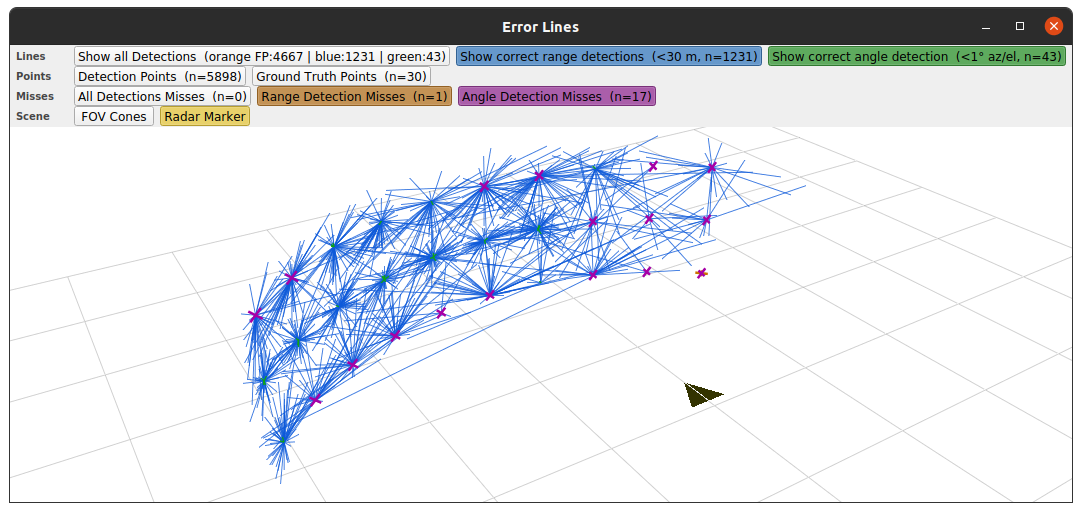
\includegraphics[width=0.9\textwidth]{integration_setup.png}
    \caption[Integration experiment ground truths and detections.]{The setup of the integration 
    stage experiment for accuracy evaluation. The figure shows the detections of a target 
    sweeping azimuth, elevation and range in a noisy scenario. Each line segment indicates the 
    ground truth on one end and the detection on the other. Purple crosses indicate ground 
    truths with no detections within 1 degree in azimuth and elevation of them. The triangle 
    marks the radar position and heading.}
    \label{fig:integration-setup}
\end{figure}

The results of the experiment are illustrated in Figures 
\ref{fig:integration-angle-recall-per-segment} and
\ref{fig:integration-RMS-position-error}.

\begin{figure}
    \incfig[0.9]{integration_angle_recall_per_segment}
    \caption[Recall Integration Experiment.]{Recall, the proportion of ground truths 
    with at least one detection within 1 degree in azimuth and elevation of them, of 
    the integration stage experiment as the integration length (number of chirps integrated
    together) increases, for both coherent and non-coherent integration in the six noise 
    intensities. As the integration length increases, the recall of the detections increases,
    with the coherent integration performing consistently better than the non-coherent integration
    across all noise intensities. Through coherent integration of 64 chirps, the recall in the 
    worst noise regime increased from near 0 to 0.9.}
    \label{fig:integration-angle-recall-per-segment}
\end{figure}

\begin{figure}
    \incfig[0.9]{integration_RMS_position_error}
    \caption[Position Error Integration Experiment.]{RMS position error of the integration 
    stage experiment as the integration length (number of chirps integrated together) increases, 
    for both coherent and non-coherent integration in the six noise intensities. The figure 
    shows that integration directly improves position accuracy, with coherent integration 
    performing slightly better than non-coherent integration when the 
    integration length is larger than 4. }
    \label{fig:integration-RMS-position-error}
\end{figure}


\FloatBarrier
\section{Constant False Alarm Rate}
\subsection{Correctness}
Under the assumption of an 8-degrees of freedom chi-squared distribution of sample noise 
power for a given quadruplet of receivers, the CFAR threshold coefficient $\alpha$ is 
calculated numerically for a range of false alarm 
rates. The actual false alarm rate is then measured by running the CFAR algorithm on a noise-only
synthetic dataset. Figure \ref{fig:alpha-cfar-results} illustrates the results.

\begin{figure}[htbp]
    \centering
    \incfig[0.4]{pfa_comparison} 
    \caption[Actual vs desired false alarm rate validating the numerical CFAR threshold.]{The actual 
    false alarm rate closely matches the desired false alarm rate across a range
    of false alarm rates. The numerical solution for $\alpha$ is therefore accurate under the assumption
    of an 8-degrees of freedom chi-squared distribution of sample noise power across a quadruplet of 
    receivers.}
    \label{fig:alpha-cfar-results}
\end{figure}

The results indicate that the numerical solution for $\alpha$ is accurate, with the actual false alarm 
rate closely matching the desired. The successful performance of CFAR with a false alarm rate of 
\(0.001\) is illustrated in Figure \ref{fig:cfar-0.001-waterfall}.

\begin{figure}[htbp]
    \centering
    \incfig[0.8]{cfar-0.001-waterfall}
    \label{fig:cfar-0.001-waterfall}
    \caption[CFAR waterfall at false alarm rate of 0.001.]{CFAR with a desired false alarm rate of \(0.001\) infrequently detects peaks in what is
    predominantly noise, as expected. The figure is a waterfall plot, with chirp on the y-axis and range
    on the x-axis. The brightness of the cell reflects the power of the corresponding chirp's range bin.
    The black space indicates that most cells are masked by CFAR.} 
\end{figure}

\subsection{Computational Performance}
The speed of each of the three CFAR implementations is measured across a range of buffer sizes, from 
one frame of 767 samples, to 4042 frames of 767 samples. This sweep is performed on both the desktop 
and the Xavier. The results are illustrated in Figures \ref{fig:cfar-implementation-performance-Xavier} 
and \ref{fig:cfar-implementation-performance-desktop}.

\begin{figure}[htbp]
    \centering
    \includesvg[width=0.75\linewidth]{CFAR implementation speed on desktop.svg} 
    \caption[CFAR implementation speed vs buffer size on the desktop.]{Computational Performance of three CFAR implementations as a function of buffer size on the
    desktop setup. The CPU implementation with a prefix sum tables is the fastest for small buffer sizes,
    but the GPU implementation is slightly faster for larger buffer sizes. The naive CPU implementation
    is the slowest across all buffer sizes.}
    \label{fig:cfar-implementation-performance-desktop}
\end{figure}

\begin{figure}[htbp]
    \centering
    \includesvg[width=0.75\linewidth]{CFAR implementation speed on Xavier.svg} 
    \caption[CFAR implementation speed vs buffer size on the Xavier.]{Computational Performance of three CFAR implementations as a function of buffer size on the
    Xavier NX setup. The CPU implementation with a prefix sum tables is the fastest for small buffer sizes,
    but the GPU implementation is slightly faster for larger buffer sizes. The naive CPU implementation
    is the slowest across all buffer sizes.}
    \label{fig:cfar-implementation-performance-Xavier}
\end{figure}

The speed is also plotted as a function of the number of CFAR training cells. The results are illustrated 
in Figures \ref{fig:cfar-implementation-performance-Xavier-training-cells} and 
\ref{fig:cfar-implementation-performance-desktop-training-cells}. The desktop results illustrate that both
the GPU and the prefix sum table implementations are not significantly affected by the number of training
cells, while the naive CPU implementation's speed increases linearly with the number of training cells. 
The Xavier results illustrate that while the prefix sum table implementation remains invariant to the 
number of training cells (as we expect), the GPU implementation's speed does increase with the number 
of training cells, due to the fact that each thread has more work to do to calculate the noise statistic. 
Results on the Xavier show that the GPU implementation is faster than either CPU implementation 
for window sizes within the practical range of 10 - 100 training cells.  

\begin{figure}
    \centering
    \includesvg[width=0.8\linewidth]{CFAR implementation speed over window size 10.svg} 
    \caption[CFAR implementation speed vs training cells on the desktop.]{Computational Performance of three CFAR implementations as a function of the number of
    training cells on the Desktop Setup. Buffer size is fixed at 10 quadruplet chirps per frame.}
    \label{fig:cfar-implementation-performance-desktop-training-cells}
\end{figure}

\begin{figure}
    \centering
    \includesvg[width=0.8\linewidth]{CFAR implementation speed over window size 10 Xavier.svg} 
    \caption[CFAR implementation speed vs training cells on the Xavier.]{Computational Performance of three CFAR implementations as a function of the number of
    training cells on the Xavier Setup. Buffer size is fixed at 10 quadruplet chirps per frame.}
    \label{fig:cfar-implementation-performance-Xavier-training-cells}
\end{figure}

Three implementations of CFAR, CA-CFAR, GO-CFAR, and SO-CFAR, were tested on the DS2 dataset with
six different noise intensities: no noise, -20, -10, 0, 10 and 20dB SNR. Figure 
\ref{fig:cfar-recall} illustrates the recall, the number of 
ground truth range bins with a detection within them, and clutter to signal
ratio as a function of noise and CFAR algorithm. Figure \ref{fig:cfar-clutter-to-signal} 
illustrates the clutter to signal ratio of each of the CFAR algorithms as noise increases, 
and Figure \ref{fig:cfar-position-error} illustrates the RMS position error of the true 
positives of each of the CFAR algorithms as noise increases.  

\begin{figure}
    \centering
    \incfig[0.8]{cfar_recall} 
    \caption[CFAR recall vs noise and algorithm.]{Recall of three CFAR algorithms as a 
    function of noise. The figure shows that the recall decreases with increasing noise, 
    and that CA-CFAR features the lowest clutter power for the noisiest regimes.}
    \label{fig:cfar-recall}
\end{figure}

\begin{figure}
    \centering
    \incfig[0.8]{cfar_clutter_to_signal} 
    \caption[CFAR clutter to signal ratio vs noise and algorithm.]{Clutter to signal 
    ratio of three CFAR algorithms as a function of noise. The figure shows that the 
    clutter to signal ratio increases with increasing noise, and that CA-CFAR 
    features the lowest clutter power for the noisiest regimes, while GO-CFAR 
    performs well in the low noise intensities.}
    \label{fig:cfar-clutter-to-signal}
\end{figure}

\begin{figure}
    \centering
    \incfig[0.8]{cfar_position_error} 
    \caption[CFAR position error vs noise and algorithm.]{RMS position error of the 
    true positives of three CFAR algorithms as a function of noise. The figure shows 
    that the position error increases with increasing noise, and that all CFAR 
    algorithms perform with similar accuracy. CA-CFAR features slightly better 
    accuracy in the noisiest regimes }
    \label{fig:cfar-position-error}
\end{figure}

\subsection{Clustering}
The clustering stage is validated on the DS2 dataset with no noise. The ground truths are 
depicted in Figure \ref{fig:angle-3d-plot}. The results are illustrated
in Figure \ref{fig:clustering-results}. The figure shows that the clustering stage successfully
maps contiguous blocks of detected range bins into single detections with continuous
range. 

\begin{figure}
    \centering
    \incfig[0.9]{cluster-experiment}
    \caption[Clustering results on the DS2 dataset with no noise.]{Clustering results on the 
    DS2 dataset with no noise. The figure shows that the clustering stage successfully
maps contiguous blocks of detected range bins into single detections with continuous
range. The y-axis is time and the x-axis is range. The colour is amplitude. The bright 
pink line in the first two subplots corresponds to the green and yellow line in the cluster 
output.}
    \label{fig:clustering-results}
\end{figure}


\subsection{Monopulse Angle Sensing}
\subsection{Correctness}
With the same DS2 dataset from the CFAR evaluation with 0 noise, the monopulse angle sensing 
algorithm is validated by comparing it's azimuth and elevation estimates to the ground truth. 
The results are illustrated in Figures \ref{fig:angle-polar-error} and 
\ref{fig:angle-3d-plot}. Seeing low error suggests that the monopulse angle sensing is 
correctly applying the reverse transformation that the radio wave simulation piece utilised
to convert position to multi-change signal data. 

\begin{figure}
    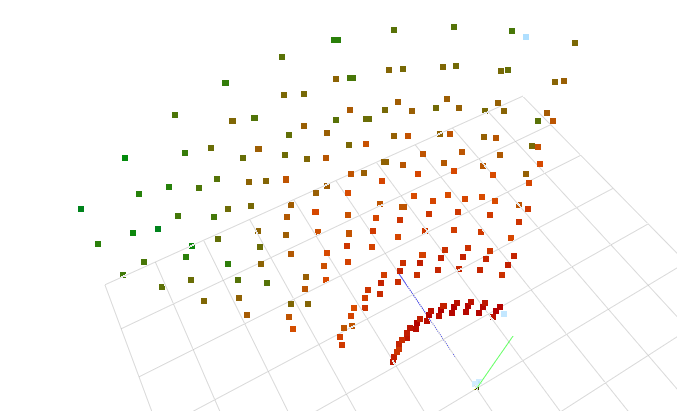
\includegraphics[width=0.8\textwidth]{angle-ground-truth-3d.png}
    \centering
    \caption[Angle experiment Ground Truth 3D plot]{The ground truth measurements of the angle sensing DS2
    dataset plotted in 3D. Points are coloured by signal strength and points are arranged in a 
    polar array.}
    \label{fig:angle-3d-plot}
\end{figure}

\begin{figure}
    \incfig[0.8]{angle_polar_error_scatter_plot}
    \centering
    \caption[Monopulse angle sensing polar error scatter plot.]{Polar error scatter plot
    of the monopulse angle sensing algorithm on the DS2 dataset with 0 noise. The figure 
    shows that the polar error of the angle estimates is generally below 0.3 degrees in 
    az el and rng and the range error is less than 1.5 meters over the tested range. } 
    \label{fig:angle-polar-error}
\end{figure}

Under -10dB SNR, the 3D plot view fills up with clutter and angle sensing accuracy 
quickly degrades. But plotting the amplitude of the detections and accumulating 
detections over 64 chirps per grid position in the dataset, clusters around the 
true target positions can be visually identified, validating the effectiveness of 
monopulse angle sensing in high noise conditions (calculated azimuth and elevation
seem to be unbiased estimators of the true azimuth and elevation). The phenomenon 
is illustrated in Figure \ref{fig:angle-3d-plot-noise}.

\begin{figure}
    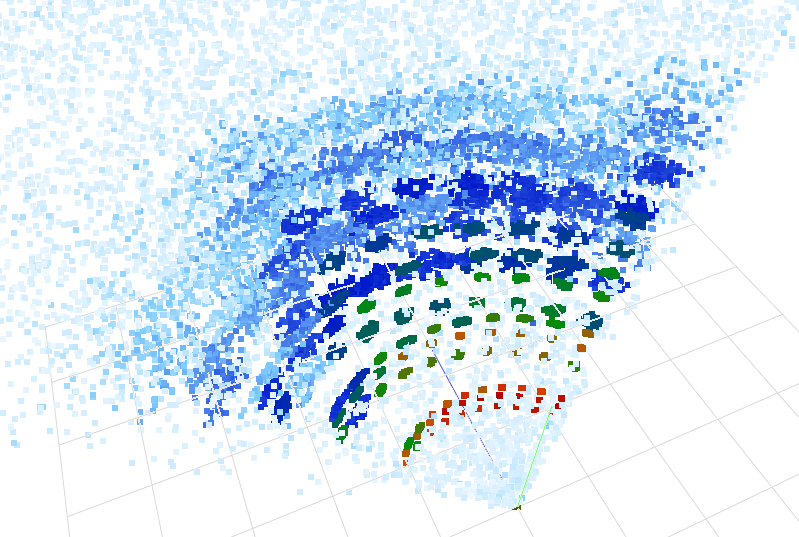
\includegraphics[width=0.7\linewidth]{angle squares light mode noisy.png}
    \caption[Monopulse angle sensing 3D plot with noise.]{3D plot of the monopulse 
    angle sensing algorithm on the DS2 dataset with -10dB SNR at max range. The 
    figure shows the 
    degradation in angle sensing accuracy under high noise conditions as range increases}
    \label{fig:angle-3d-plot-noise}
\end{figure}

To understand the failure modes of monopulse angle sensing for multiple targets, 
a simulation tool was built to validate the monopulse angle sensing algorithm on 
synthetic data. The tool allows the 
user to create multiple targets, and specify the bearing/elevation ratios of each 
target. The simulated data is then 
processed by the preprocessing subsystem, the aggregator, CFAR, and the monopulse 
angle sensing algorithm. The 
resulting angle estimates are visualised live in a 3D plot. A frame of this view is 
illustrated in Figure 
\ref{fig:monopulse-angle-sensing-results}.

\begin{figure}
    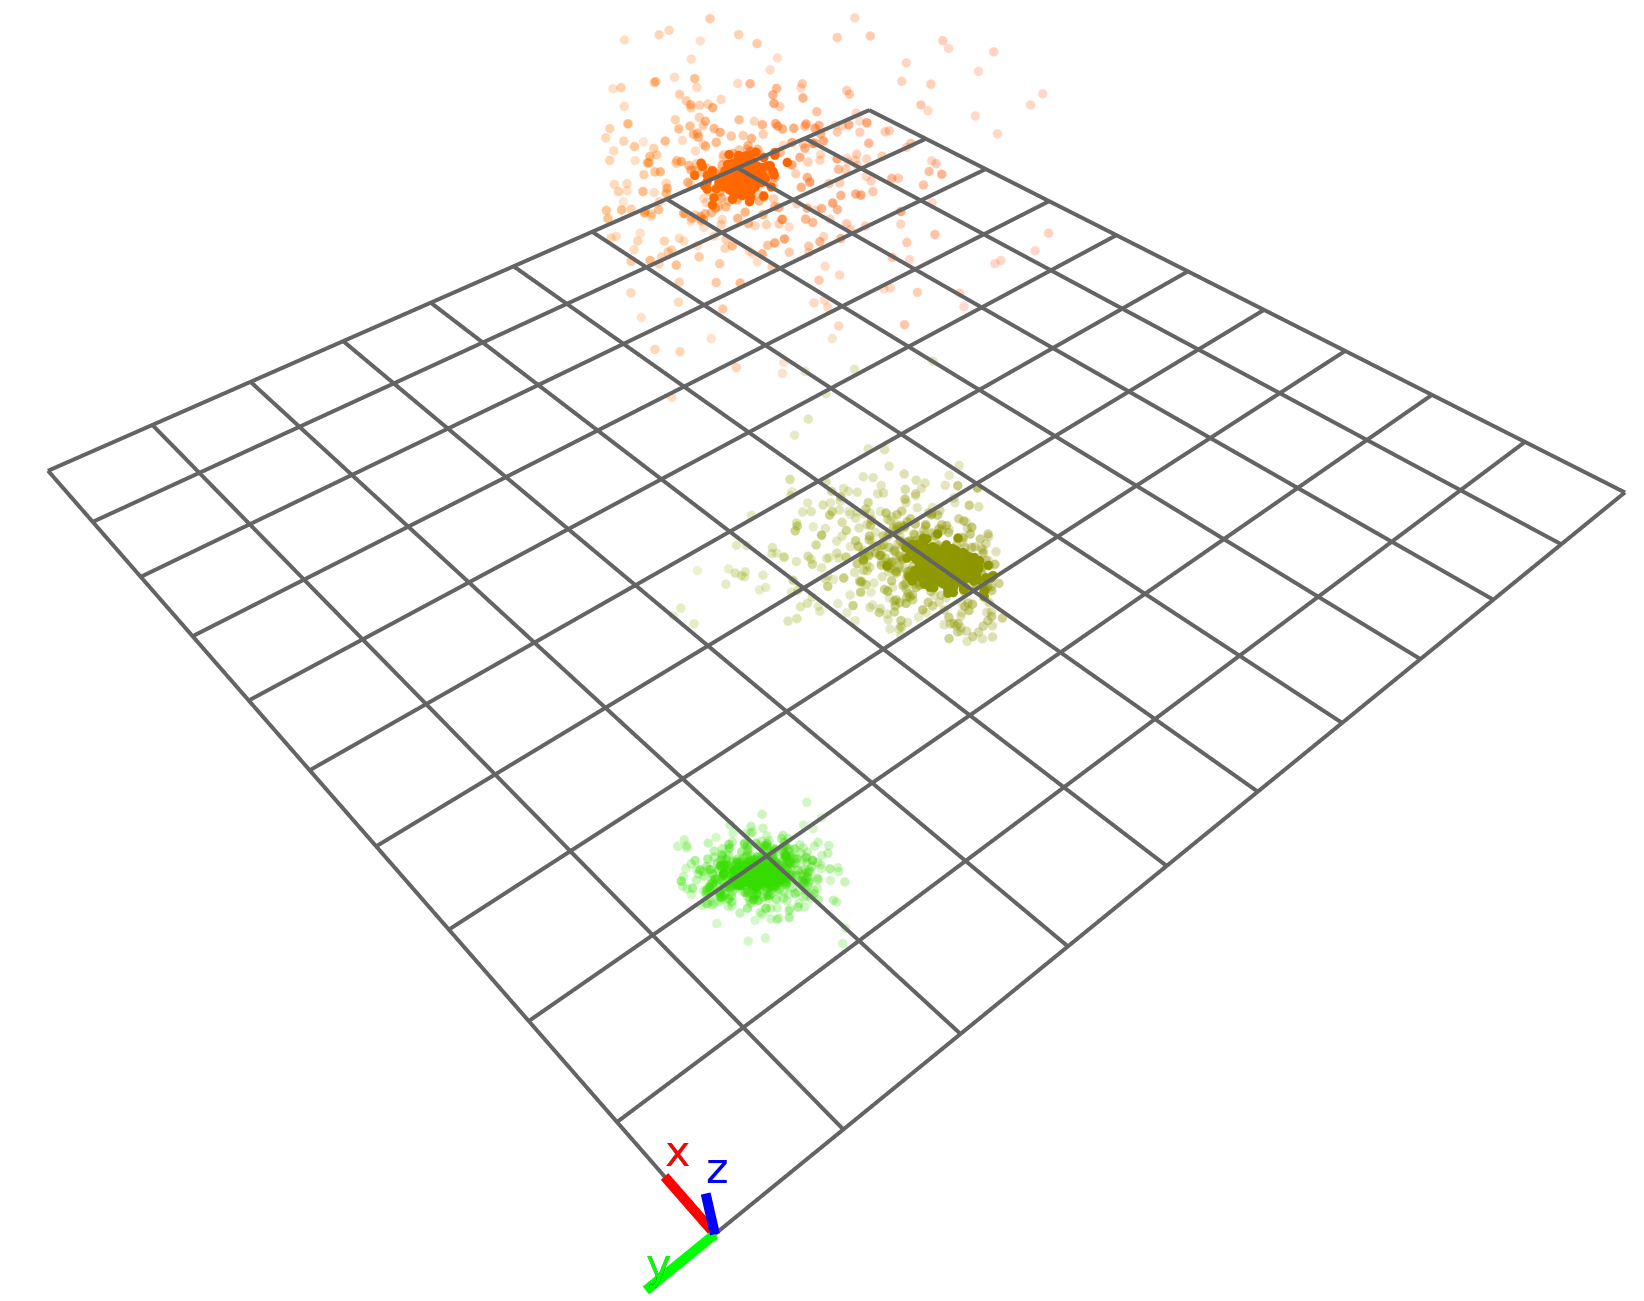
\includegraphics[width=0.8\linewidth]{monopulse_angle_sensing_results.png}
    \caption[Monopulse angle sensing results on synthetic data.]{Results of the monopulse angle sensing algorithm on synthetic data. The colour of the dots indicate
    the range of the detections, with green being close and orange being far away. The opacity of the dots indicate
    the strength of the detections, with more opaque dots being stronger. The plot features the most recently 1000
    detections. The spread of the dots increases with range as expected, and the
    upper and lower bounds of elevation and bearing match the field of view
    defined by the calibration polynomial.}
    \label{fig:monopulse-angle-sensing-results}
\end{figure}

The relative latency cost of the angle and CFAR operations were measured through an ablation study on the detection 
subsystem. The results are illustrated in Figure \ref{fig:tracking-latency-trials} which shows the latency 
of just CFAR, just angle sensing, and both, and Figure \ref{fig:tracking-latency-breakdown}. 

\begin{figure}
    \includesvg[width=0.8\linewidth]{tracking_latency_trials.svg}
    \caption[Detection subsystem latency for CFAR, angle sensing, and both.]{Latency of the subsystem running CFAR, angle sensing, and both on a log scale.
    The latency of the subsystem
    running CFAR is similar to the latency of the subsystem running both, while angle sensing
    is 1.5-5 times faster than either,
    suggesting that CFAR dominates the latency of the subsystem.}
    \label{fig:tracking-latency-trials}
\end{figure}

\begin{figure}
    \includesvg[width=0.8\linewidth]{tracking_latency_breakdown.svg}
    \caption[Detection subsystem latency breakdown from ablation study.]{A breakdown of the latency of the subsystem estimated from the ablation study.
    Most of the latency is split
    between CFAR and the overhead of handling the data, which involves synchronising threads
    and migrating data between the CPU and GPU.}
    \label{fig:tracking-latency-breakdown}
\end{figure}

The angle stage has no parameters to tune other than the coefficients of the calibration
polynomial, which are determined by the beam shape of the receivers. Therefore, the latency 
and correctness analysis is all that can be done. 

\subsection{Tracking}
To validate the tracking stage, 12 scenarios were selected from the DS2 dataset. 
These scenarios involve 1, 2 and 3 targets at no noise, -20, -10, and 0 SNR. Figures 
\ref{fig:tracking-initiation-accuracy} and \ref{fig:tracking-position-accuracy} 
demonstrate the effect of noise and target count on track initiation accuracy, 
position accuracy, and track health.  

%include 4 figures
% track_basic_stats
% track_MOTA_stats
% track_RMS Angle Error
% track_RMS Distance

\begin{figure}
    \incfig[1]{track_basic_stats}
    \caption[Tracking initiation accuracy and track health.]{Tracking accuracy and 
    track health across 12 scenarios with different noise and target count. The figure shows 
    that track-level accuracy, precision, recall, are highest when there is some noise, and 
    only one target. Point level accuracy, precision and recall are also highest in that 
    scenario.}
    \label{fig:tracking-initiation-accuracy}
\end{figure}

\begin{figure}
    \incfig[1]{track_MOTA_stats}
    \caption[Tracking MOTA (Multi-Object Tracking Accuracy) statistics.]{MOTA is highest in the presence of some 
    noise and one target. MOTP (Multi-Object Tracking Precision) strictly increases with noise for all target 
    counts. Mean completeness, mean delay until initiation, fragmentation, and survival 
    ratio are also depicted. }
    \label{fig:tracking-position-accuracy}
\end{figure}

\begin{figure}
    \incfig[0.8]{track_RMS_Angle_Error}
    \caption[Tracking RMS angle error.]{Tracking RMS angle error across 12 scenarios 
    with different noise and target count. The figure shows that RMS angle error 
    degrades with increasing noise and target count.}
    \label{fig:tracking-angle-error}
\end{figure}

\begin{figure}
    \incfig[0.8]{track_RMS_Distance}
    \caption[Tracking RMS distance error.]{Tracking RMS distance error across 12 scenarios 
    with different noise and target count. The figure shows that RMS distance error 
    degrades with increasing noise and target count.}
    \label{fig:tracking-distance-error}
\end{figure}

% Here include basic stats and fancy stats. 
% Talk more about random targets instead of sweep
% Show the ground truth for three targets and some view-tracks.py images. 
% Get everyone to understand how much the tracking stage is doing.


